%Copyright 2019 Christopher M. Jermaine (cmj4@rice.edu) and Risa B. Myers (rbm2@rice.edu)
%
%Licensed under the Apache License, Version 2.0 (the "License");
%you may not use this file except in compliance with the License.
%You may obtain a copy of the License at
%
%    https://www.apache.org/licenses/LICENSE-2.0
%
%Unless required by applicable law or agreed to in writing, software
%distributed under the License is distributed on an "AS IS" BASIS,
%WITHOUT WARRANTIES OR CONDITIONS OF ANY KIND, either express or implied.
%See the License for the specific language governing permissions and
%limitations under the License.
%===============================================================
\documentclass[aspectratio=169]{beamer}
\mode<presentation> 
{
\usetheme[noshadow, minimal,numbers,riceb,nonav]{Rice}
\usefonttheme[onlymath]{serif}
\setbeamercovered{transparent}
}
\useinnertheme{rectangles}

\usepackage[english]{babel}

\usepackage{amsmath}
\usepackage{mathptmx}
\usepackage{helvet}
\usepackage{courier}
\usepackage[T1]{fontenc}
\usepackage{trajan}
\usepackage{ textcomp }
\renewcommand{\footnotesize}{\tiny}


\usepackage{listings}

\newenvironment{noindentitemize}
{ \begin{itemize}
 \setlength{\itemsep}{1.5ex}
  \setlength{\parsep}{0pt}   
  \setlength{\parskip}{0pt}
 \addtolength{\leftskip}{-2em}
 }
{ \end{itemize} }

\newenvironment{noindentitemize2}
{ \begin{itemize}
  \setlength{\itemsep}{0ex}
  \setlength{\parskip}{0pt}
  \setlength{\parsep}{0pt}   
  \addtolength{\leftskip}{-2em}  }
{ \end{itemize} }

\lstnewenvironment{SQL}
  {\lstset{
        aboveskip=5pt,
        belowskip=5pt,
        escapechar=!,
        mathescape=true,
        upquote=true,
        language=C,
        basicstyle=\linespread{0.94}\ttfamily\normalsize,
        deletekeywords={VALUE, PRIOR},
        showstringspaces=true}
        \vspace{0pt}%
        \noindent\minipage{0.47\textwidth}}
  {\endminipage\vspace{0pt}}
  
\newcommand{\LIKES}{\textrm{LIKES}} 
\newcommand{\FREQUENTS}{\textrm{FREQUENTS}} 
\newcommand{\SERVES}{\textrm{SERVES}} 
\newcommand{\CAFE}{\textrm{CAFE}} 
\newcommand{\COFFEE}{\textrm{COFFEE}} 
\newcommand{\DRINKER}{\textrm{DRINKER}} 
\newcommand{\ALLPEEPS}{\textrm{ALLPEEPS}} 
\newcommand{\ALLCOMBOS}{\textrm{ALLCOMBOS}} 

\setbeamerfont{block body}{size=\tiny}

%===============================================================%

\title[]
{Tools \& Models for Data Science}

\subtitle{Deep Learning with TensorFlow}

\author[]{Chris Jermaine \& Risa Myers}
\institute
{
  Rice University 
}

\date[]{}

\subject{Beamer}

\begin{document}

\begin{frame}
 \titlepage
\end{frame}
%***********************************************************
\begin{frame}{This Lecture...}

\begin{itemize}
        \item Is meant to de-mystify RNNA6.py
        \begin{itemize}
	\item RNNA6.py is the code we give you with A6
        \item Use this lecture + the Internet when you puzzle over the code
        \end{itemize}

\end{itemize}
\end{frame}
%***********************************************************
\begin{frame}{What Is TensorFlow?}

\begin{itemize}
	\item Has many components...
	\item Including a distributed computation engine
	\item But for our purposes, it is an automatic differentiation engine
        \begin{itemize}
                \item That is, you specify an ``forward'' process (the inference process)
		\item And it automatically figures out a gradient descent algorithm (the ``backward'' or learning process)
		\item Even if you have a complicated forward process, it will differentiate it for you
		\item Even something complicated like an RNN
		\item TF will also allow you to efficiently execute the backward propagation algorithm over data
        \end{itemize}
\end{itemize}

\end{frame}
%***********************************************************
\begin{frame}{How to Specific A Forward Process}

\begin{itemize}
\item You push tensors through various computations TF provides
	\begin{itemize}
	\item A ``tensor'' is a generalization of a matrix/vector
	\item Can have any number of dimensions 
	\item Tensors are TF's most fundamental data type
	\item Everything is based off of them
	\end{itemize}
\end{itemize}
\end{frame}
%***********************************************************
\begin{frame}{Data Types in TensorFlow}

\begin{itemize}
\item Use floats (32-bit representation)
	\begin{itemize}
	\item Support for doubles (64-bit) is not great
	\item Added in later in TF
	\item The extra bits are just not that important in ML
	\item Millions of neurons, working together can withstand a lot of inaccuracy from loss of precision
	\item Shorter representation can speed computation
	\end{itemize}
\end{itemize}
\end{frame}
%***********************************************************
\begin{frame}[fragile]{Two Kinds of Tensors in Forward Process}

\begin{itemize}
\item 1) Placeholders
\begin{itemize}
\item These are tensors whose value will be provided at training time
\item They are inputs into the forward process
\item Declared like 
\end{itemize}
\end{itemize}
\begin{SQL} 
inputX = tf.placeholder
  (tf.float32, [batchSize, 256 * maxSeqLen])
\end{SQL}
\begin{itemize}
\item \texttt{batchSize} = size of mini-batch used 
\item \texttt{256} = one hot encoding (256 characters)
\item \texttt{maxSeqLen} = max length of line of text
\item \texttt{[batchSize, 256 * maxSeqLen]} = 2D tensor dimensions
\end{itemize}
\end{frame}
%***********************************************************
\begin{frame}[fragile]{Two Kinds of Tensors in Forward Process}

\begin{itemize}
\item (2) Variables
\begin{itemize}
\item These are tensors whose value will be learned
\item They are computed during the backward process
\item Declared like 
\end{itemize}
\end{itemize}
\begin{SQL} 
b = tf.Variable(np.zeros((1, hiddenUnits)), dtype=tf.float32)
\end{SQL}
\begin{itemize}
\item \texttt{(1, hiddenUnits)} = initialization dimensions
\end{itemize}
\end{frame}
%***********************************************************
\begin{frame}[fragile]{Constructing the Forward Process}

\begin{itemize}
\item The forward process is specified by composing operators over tensors
\item Example:
\end{itemize}
	\begin{SQL}
next_state = tf.tanh(tf.matmul(inputPlusState, W) + b)	
	\end{SQL}
	\begin{itemize}
	\item In this line of code, operators are ``tanh'', ``matmul,'' and ``+''
	\begin{itemize}
	\item Note: TF does not actually run these operators!
	\item It remembers how you composed them
	\item And uses those computations to build the backward process later
\end{itemize}
\item \texttt{inputPlusState} = characters concatenated with the next state
\item \texttt{W} = Weight matrix
\item \texttt{b} = bias
\item Recall: The input to a layer is a matrix multiplication of the weights and the outputs from the prior layer

	\end{itemize}

\end{frame}
%***********************************************************
\begin{frame}[fragile]{Another Interesting Operation}

\begin{columns}[b]
\begin{column}{0.6\textwidth}
\begin{itemize}
\item The ``unstack'' operation
\item Example:
\end{itemize}
        \begin{SQL}
sequenceOfLetters = tf.unstack(inputX, axis=2)
        \end{SQL}
        \begin{itemize}
        \item Takes a $d$ dimension tensor 
	\item And converts it to a list of $d$, $d-1$ dimension tensors
	\item Useful if you want to iterate through a tensor
        \item In RNNA6, we want to iterate through the lines of text
        \end{itemize}
\end{column}
\begin{column}{0.4\textwidth}
%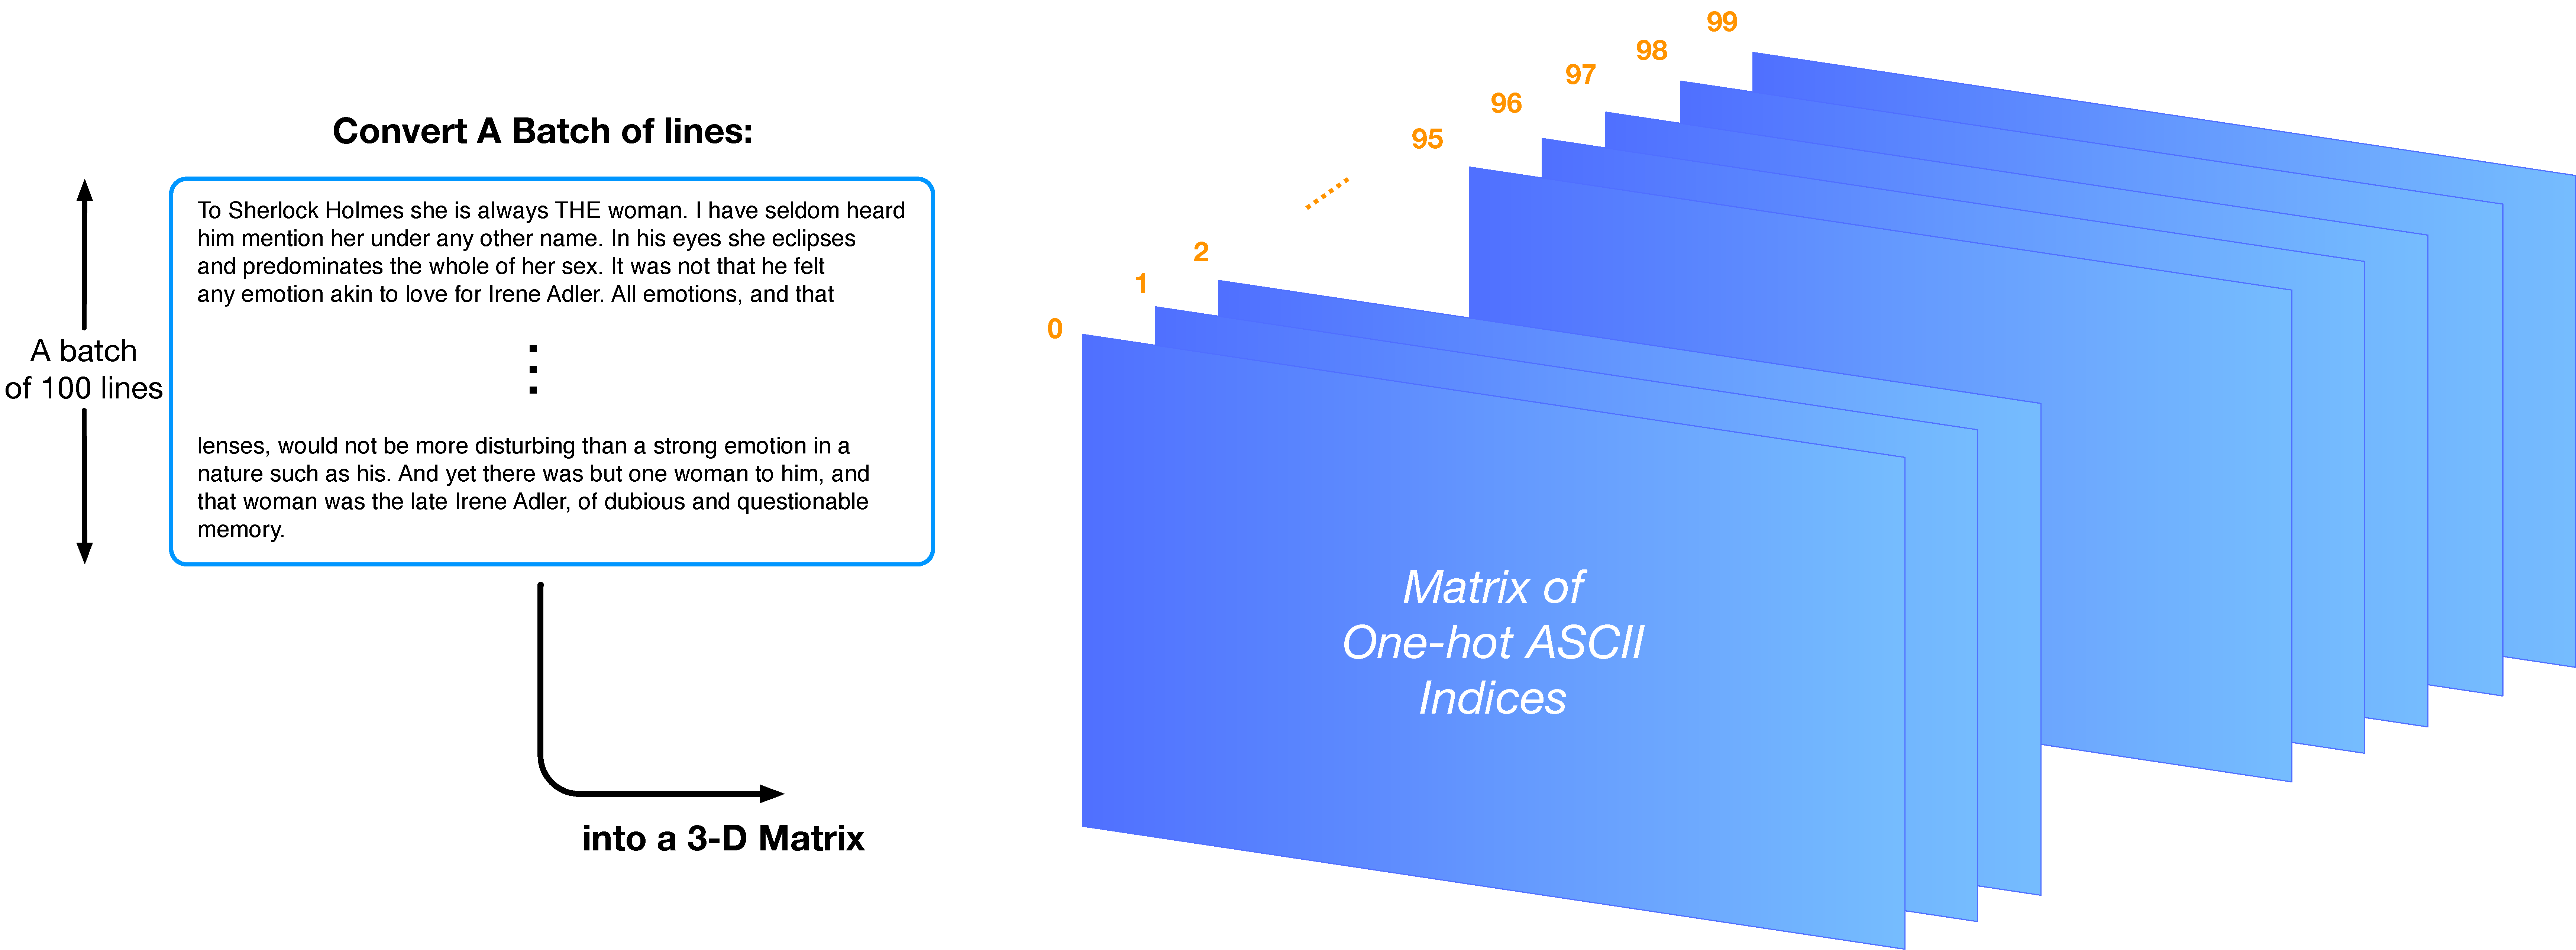
\includegraphics[width=1\textwidth]{lectTF/batch.pdf}
\end{column}
\end{columns}

\end{frame}
%***********************************************************
\begin{frame}[fragile]{Alternative to Unstack}

\begin{itemize}
\item Could have ``maxSeqLen'' different 2-$d$ tensors
\item Then would not have to unstack
\item But this may be less convenient
\end{itemize}

\end{frame}
%***********************************************************
\begin{frame}[fragile]{Input Data}

\begin{columns}
\begin{column}{0.5\textwidth}
\begin{itemize}
\item Batches of 2D tensors stored as a dictionary
\item Key: Line number (sequentially assigned)
\item Value: Pair of (class, One-hot-encoding of the character)
\item Where 
\begin{itemize}
\item Dimension 1: Character in the line
\item Dimension 2: One-hot-encoding of the character 
\item Lines are padded to make them the same length
\end{itemize}
\end{itemize}
\end{column}
\begin{column}{0.5\textwidth}
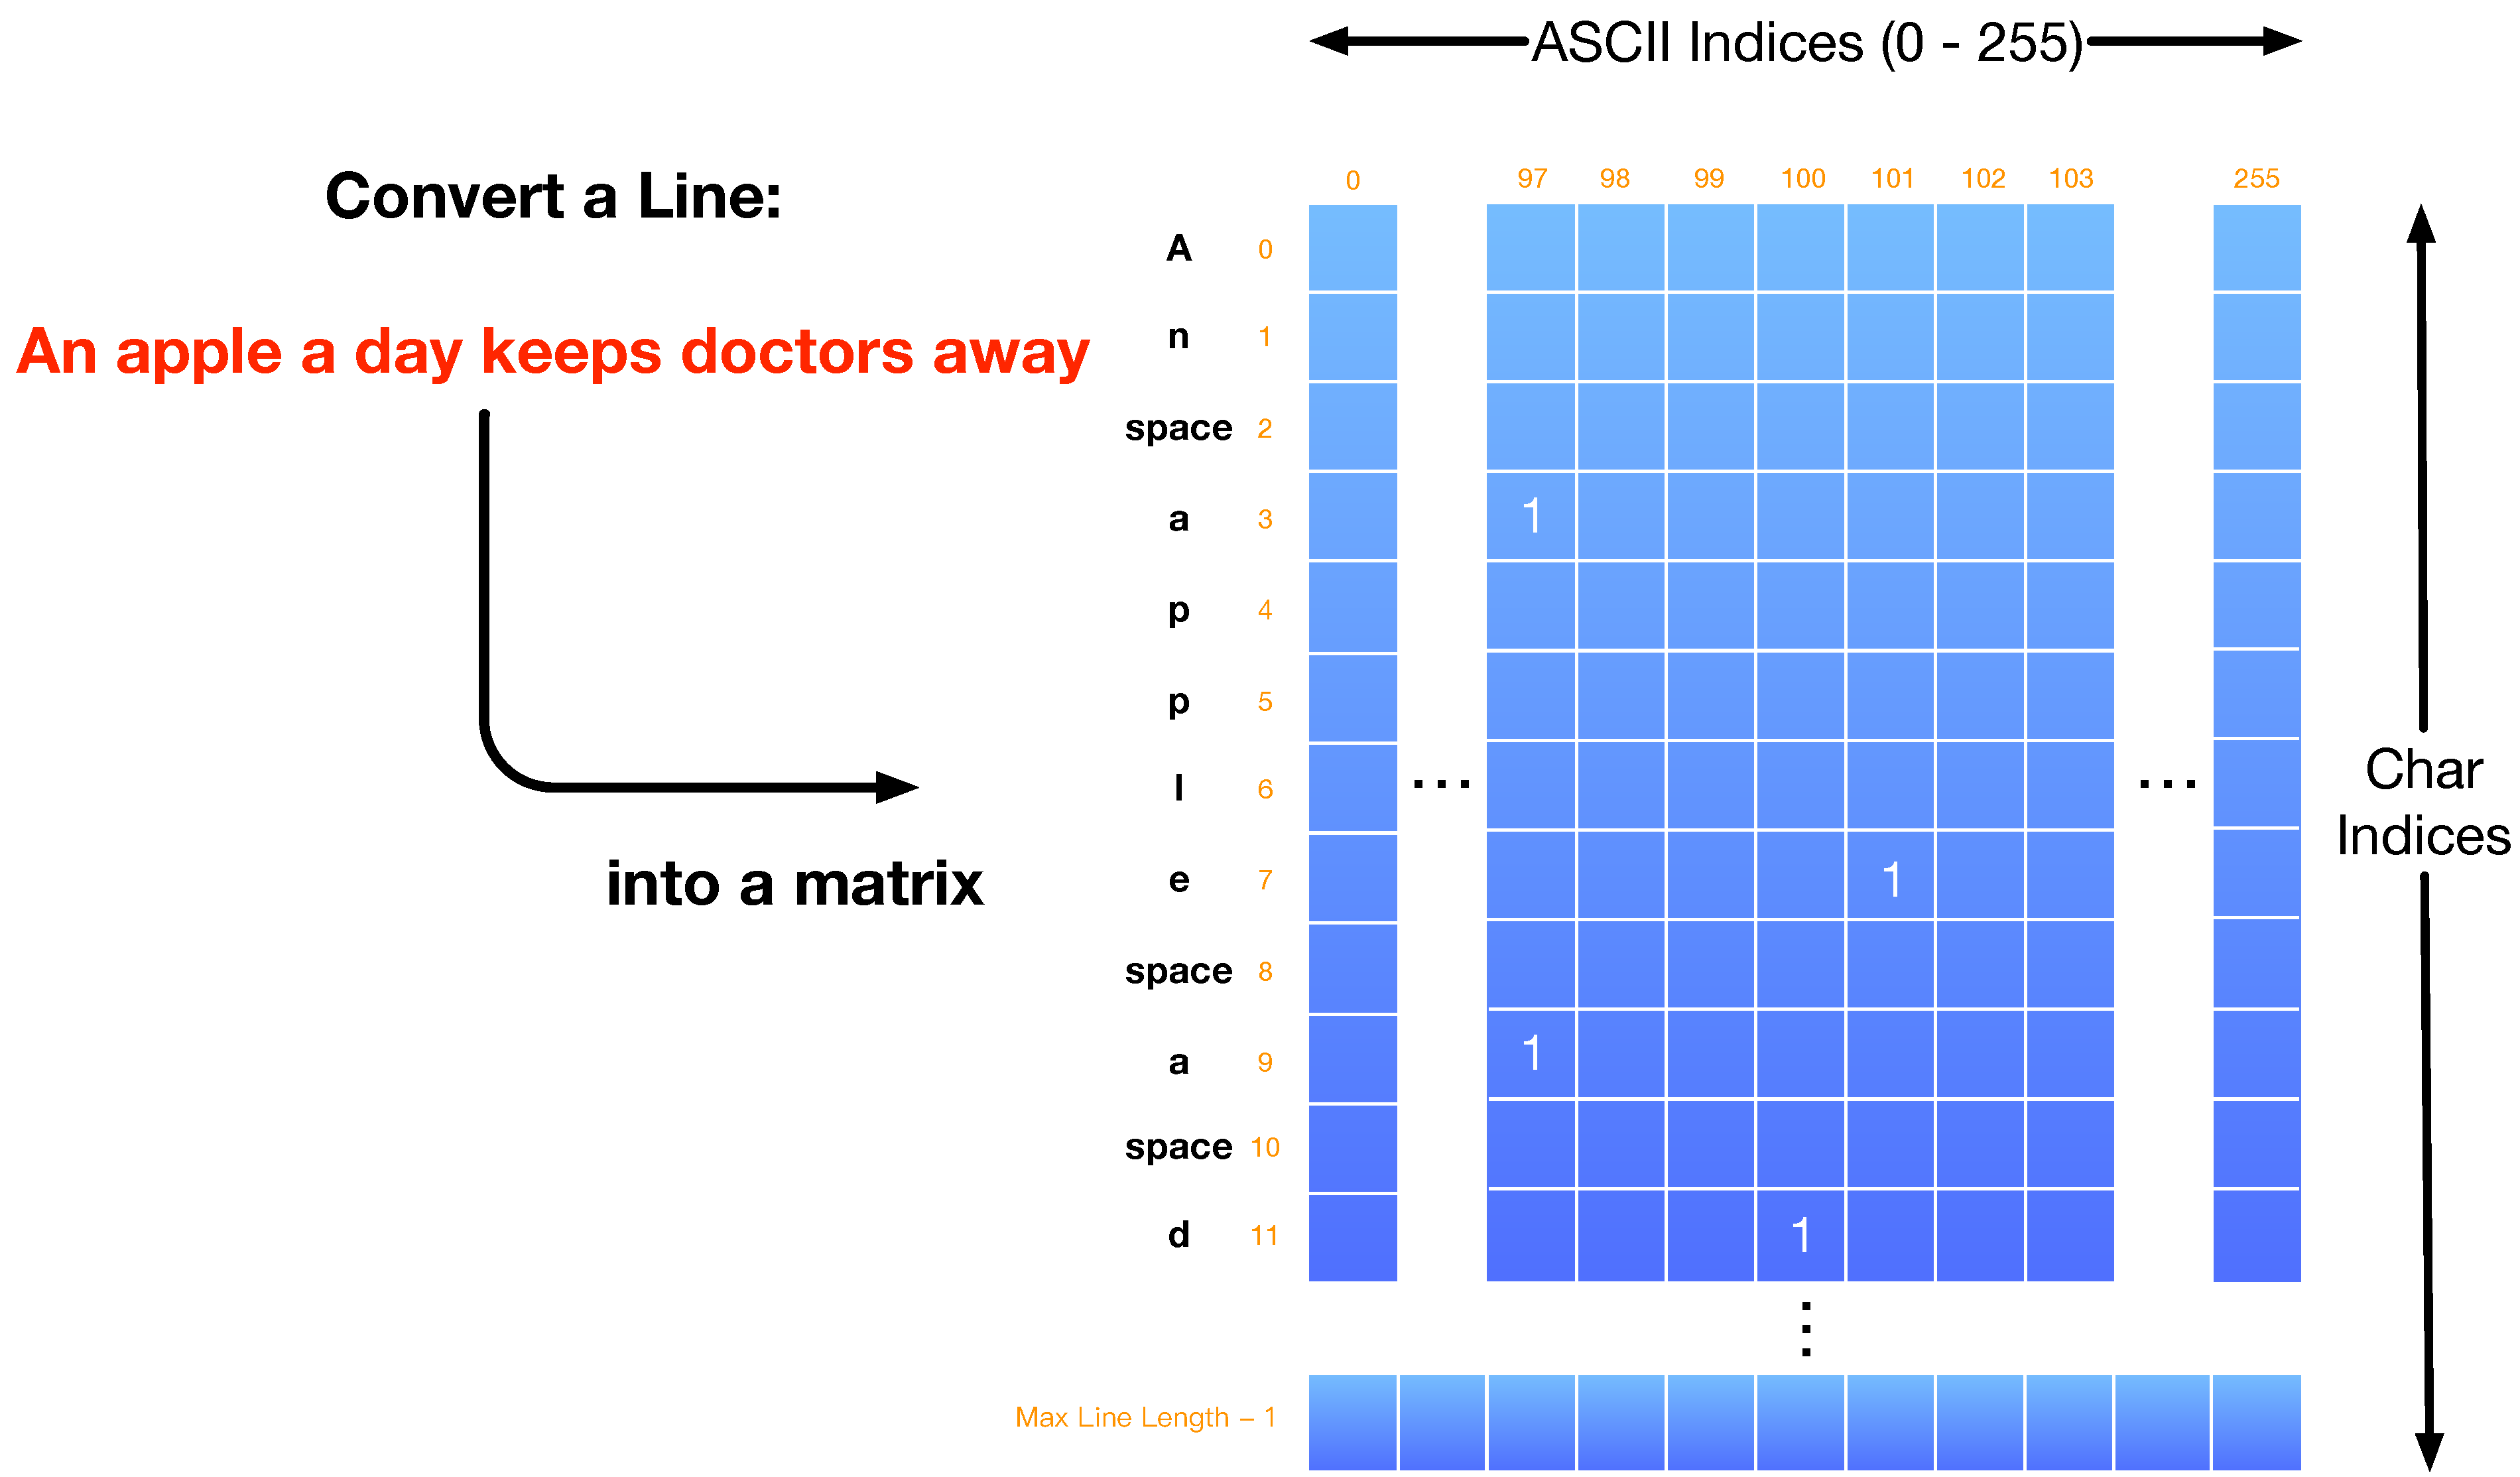
\includegraphics[width=1\textwidth]{lectTF/onehotencoding.pdf}
\end{column}
\end{columns}
\end{frame}
%***********************************************************
\begin{frame}[fragile]{Batches}

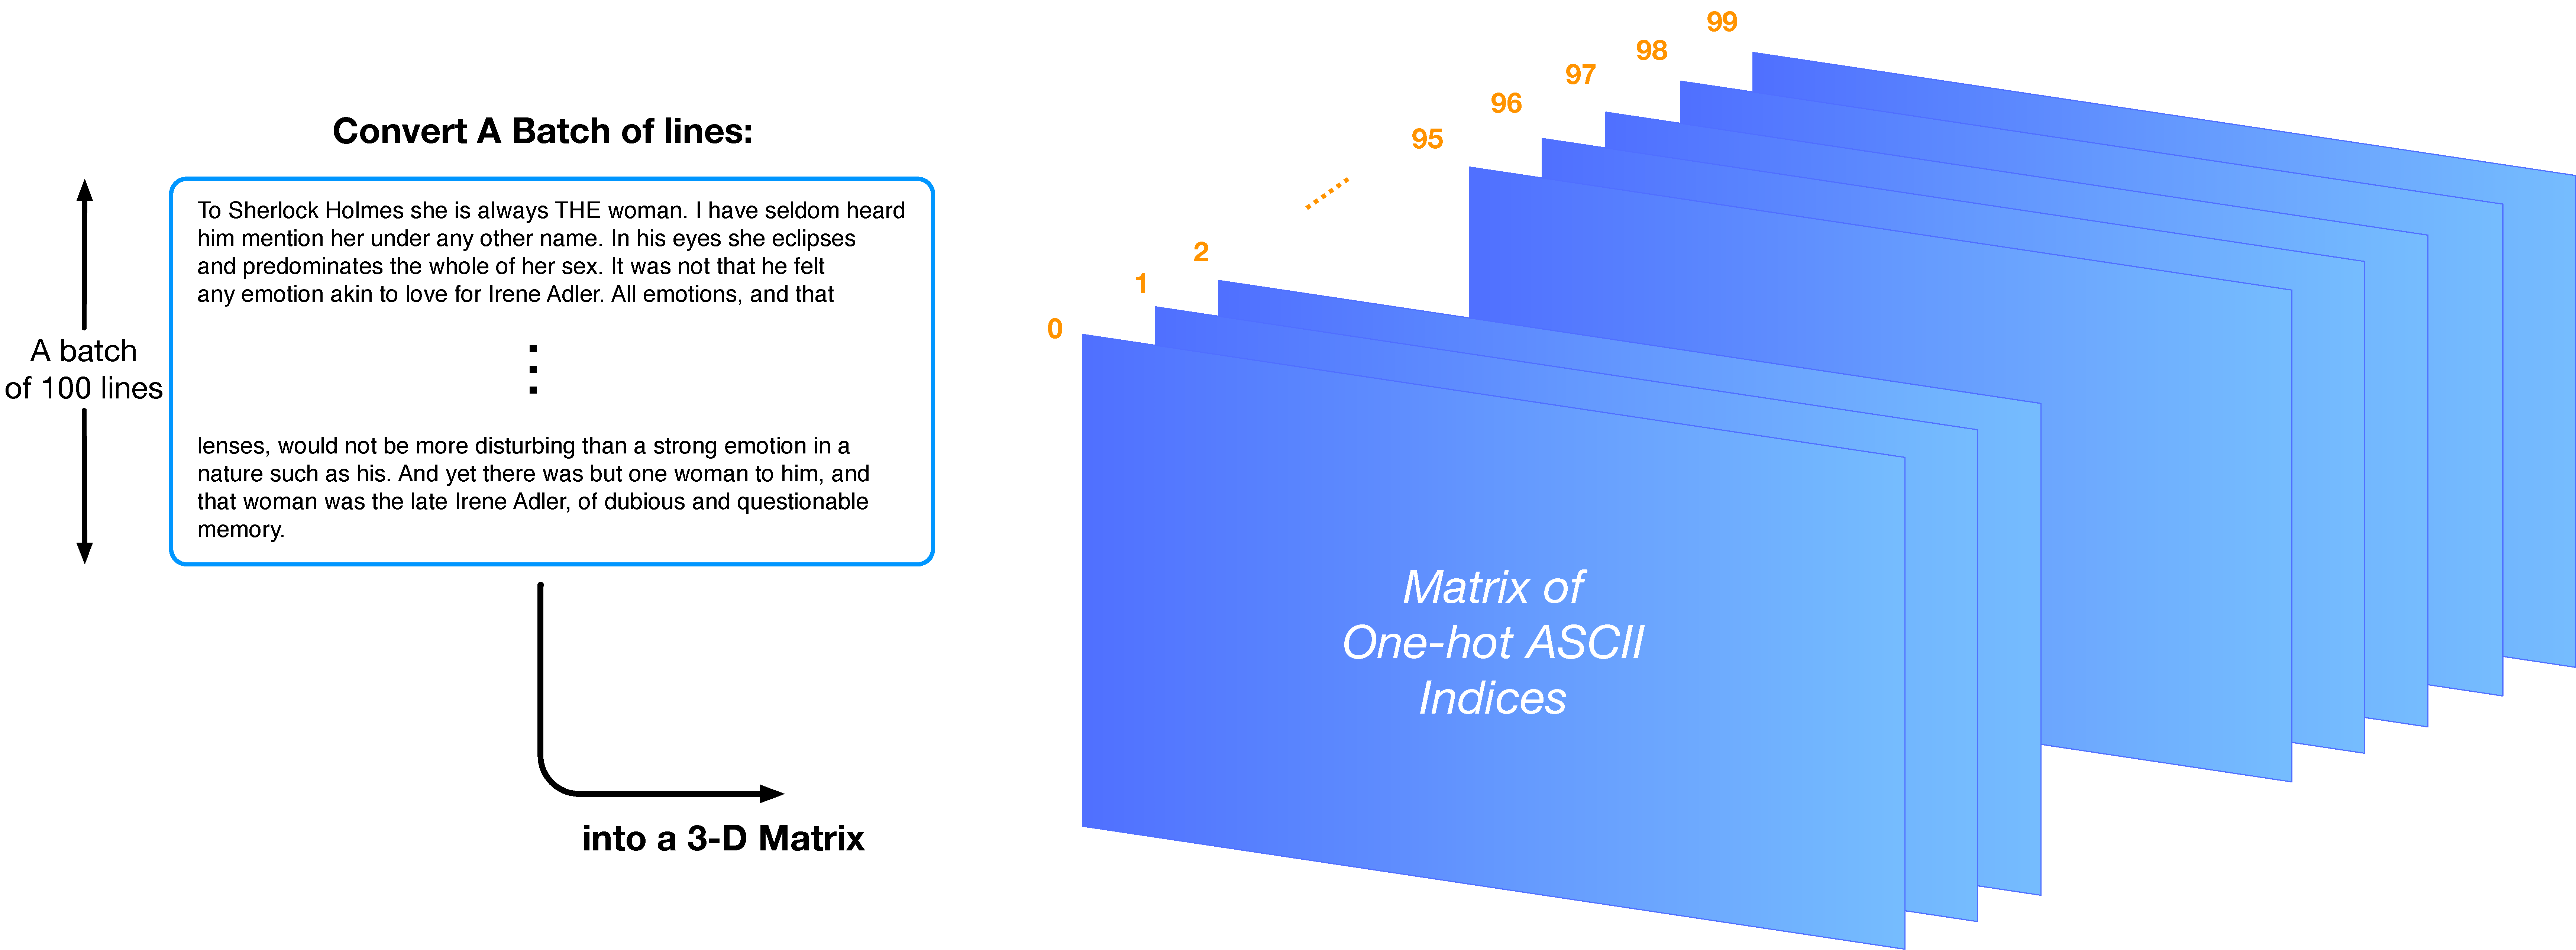
\includegraphics[width=1\textwidth]{lectTF/batch.pdf}


\end{frame}
%***********************************************************
\begin{frame}{Cross Entropy Loss for Classification}

\begin{itemize}
\item Measures how close a prediction (from a vector of probabilities) is to the actual label
\item Probabilities come from a softmax function
\item We want high probabilities to go to the correct labels
\item Cross entropy is:
$$H(p, q) = -\sum_x p(x) \log q (x)$$
\item We want to minimize it!
\item Used as the loss function in training
\end{itemize}

%http://rdipietro.github.io/friendly-intro-to-cross-entropy-loss/
\end{frame}
%***********************************************************
\begin{frame}{Cross Entropy Loss for Classification}

\begin{columns}
\begin{column}{0.5\textwidth}
\begin{itemize}
\item For probability distribution $q$ spit out by the learner
	\begin{itemize}
        \item Where (for example) $q(2) = .3$ means the learner thinks there is a $.3$ chance class is $2$
	\item And an answer distribution $p$
	\item Where $p(i) = 1$ if answer is class $i$, $0$ otherwise
	\end{itemize}
\item Cross entropy is:
$$H(p, q) = -\sum_x p(x) \log q (x)$$
\end{itemize}
\end{column}
\begin{column}{0.5\textwidth}
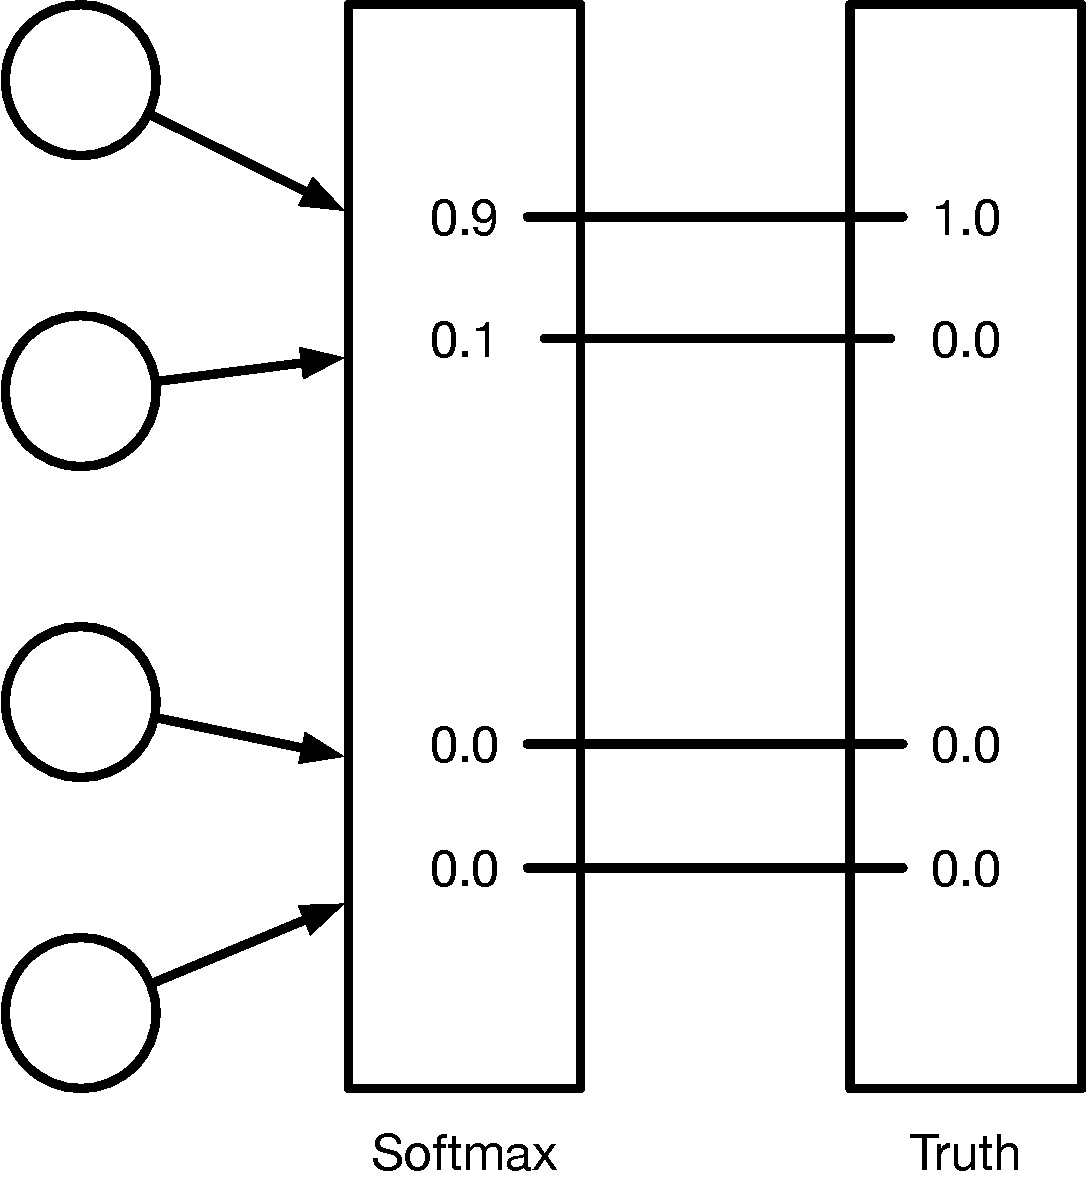
\includegraphics[width=1\textwidth]{lectTF/crossEntropy.pdf}
\end{column}
\end{columns}

%http://rdipietro.github.io/friendly-intro-to-cross-entropy-loss/
\end{frame}
%***********************************************************
\begin{frame}[fragile]{Cross-Entropy in TensorFlow}
\begin{itemize}
\item Trivially implemented in TF
\item They give you an operator for it
\end{itemize}
	\begin{SQL}
losses = tf.nn.sparse_softmax_cross_entropy_with_logits
	(logits=outputs, labels=inputY)
	\end{SQL}
	\begin{itemize}
	\item Input to function (outputs in this case) is output from tanh functions at top of the NN
	\item There should be one tanh output per class per data point
	\item Also accepts  a vector with the correct labels
	\item TF does softmax and compares predictions with the truth
	\item Then computes cross entropy
	\end{itemize}
\end{frame}
%***********************************************************
\begin{frame}[fragile]{Learning}

\begin{itemize}
\item TF has many different gradient-based algorithms to choose from
	\begin{itemize}
	\item Switching between them means changing one line of code
	\item Ex:
	\end{itemize}
\end{itemize}
	\begin{SQL}
trainingAlg = tf.train.AdagradOptimizer
     (0.02).minimize(totalLoss)
	\end{SQL}
	\begin{itemize}
	\item This (obviously) runs the Adagrad algorithm (look it up!)
	\item Alternative to gradient descent
	\item 0.02 is the learning rate
	\end{itemize}
\end{frame}
%***********************************************************
\begin{frame}[fragile]{Invoking One Iter of Gradient Descent}

\begin{SQL}
_totalLoss, _trainingAlg, _currentState, 
     _predictions, _outputs = sess.run(
    [totalLoss, trainingAlg, currentState, 
     predictions, outputs],
    feed_dict={
         inputX:x,
         inputY:y,
         initialState:_currentState
    })
\end{SQL}

\begin{itemize}
\item Args to ``run'':
	\begin{itemize}
	\item ``feed\_dict'' should tell TF what values to use for each placeholder
	\item You miss a placeholder?  TF will complain
	\item List of vars (totalLoss, trainingAlg, etc)... what are they for?
	\item Tells TF any Variables whose values you want returned
	\item Given back to you as NumPy arrays
	\end{itemize}
\end{itemize}
\end{frame}
%***********************************************************
\begin{frame}[fragile]{Invoking One Iter of Gradient Descent}

\begin{SQL}
_totalLoss, _trainingAlg, _currentState, 
     _predictions, _outputs = sess.run(
    [totalLoss, trainingAlg, currentState, 
     predictions, outputs],
    feed_dict={
         inputX:x,
         inputY:y,
         initialState:_currentState
    })
\end{SQL}

\begin{itemize}
\item \texttt{sess.run}: 1 iteration
\item \texttt{\_currentState}: numpy matrix of hidden states; all zeros initially, 1st value for hidden states
\item Watch the values of the tensors returned
\end{itemize}
\end{frame}
%***********************************************************
\begin{frame}[fragile]{Accessing Variables}

\begin{itemize}
\item Just ask ``run'' to return it 
\begin{itemize}
	\item Like in last slide
	\item Or, just use
\end{itemize}
\end{itemize}
\begin{SQL}
sess.run (W)
\end{SQL}
\begin{itemize}
	\item Will return last val of W as a NumPy array
\end{itemize}
\end{frame}
%***********************************************************
\begin{frame}[fragile]{Saving Sessions}

\begin{itemize}
\item When a training session ends, it is gone
\item But you can save it
\end{itemize}
\begin{SQL}
saver = tf.train.Saver() 
saver.save(sess, 'checkPoint.tf')
\end{SQL}
\begin{itemize}
\item Then later can load it up again
\end{itemize}
\begin{SQL}
sess = tf.Session()
saver = tf.train.Saver()
saver.restore(sess, 'checkPoint.tf')
\end{SQL}
\begin{itemize}
\item Very useful!!
\end{itemize}
\end{frame}
%***********************************************************
\begin{frame}[fragile]{My Code Doesn't work!}

\begin{itemize}
\item Make sure your NN is correctly connected
\begin{itemize}
\item Check sizes and shapes of tensors
\item Check the input data
\end{itemize}
\item Monitor the objective function / loss
\item Check the initialization (note small variance)
\item Check the number of hidden units
\item Print out information at each iteration
\item Restructure the code to be able to work with it interactively
\end{itemize}
\end{frame}
%***********************************************************
\begin{frame}{Questions?}
\end{frame}
\end{document}
